\section{Task 1}
Să se creeze două viziuni ı̂n baza interogărilor formulate ı̂n două exercit, ii indicate din capitolul
4. Prima viziune să fie construită ı̂n Editorul de interogări, iar a doua, utilizı̂nd View Designer.
\begin{figure}[H]
	\centering
		\minipage{0.48\textwidth}
		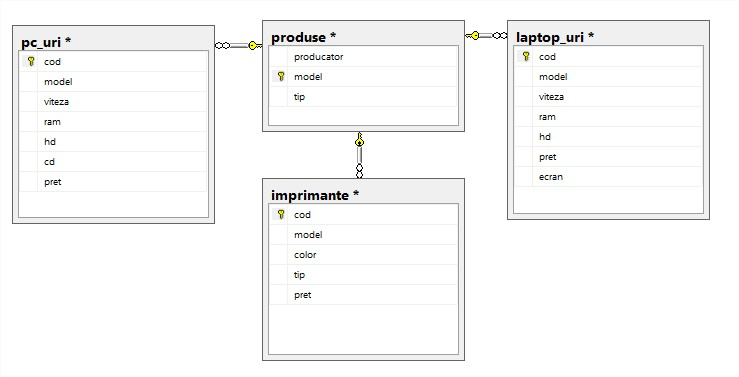
\includegraphics[width=\linewidth]{screens/1.jpg}
		\caption*{Figure 1: Diagram creation}
		\label{}
	\endminipage\hfill
\end{figure}

\section{Task 2}
Creați în baza de date calculatoare definită în lucrările anterioare, trei scheme noi: stoc, pc\_laptop și copiatoare.

\begin{figure}[H]
	\centering
	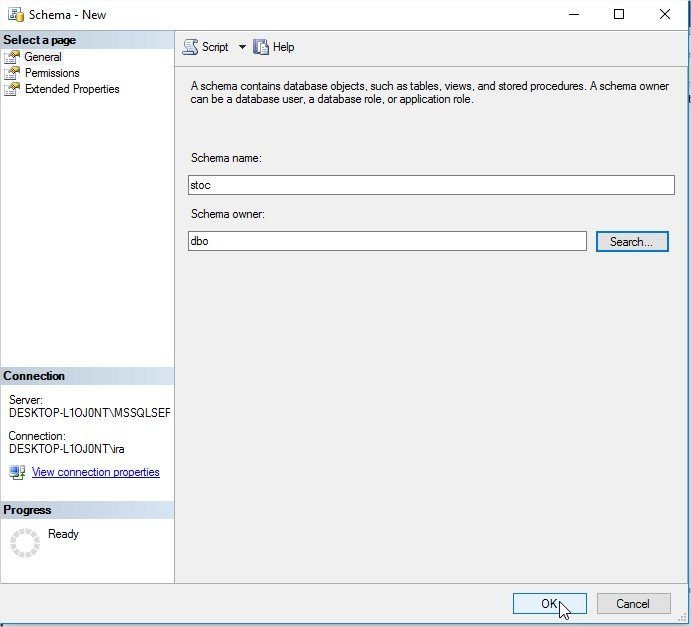
\includegraphics[scale=0.4]{screens/3.jpg}
	\caption*{Figure 2: Defining schema for stoc}
	\label{}
\end{figure}

\begin{figure}[H]
	\centering
	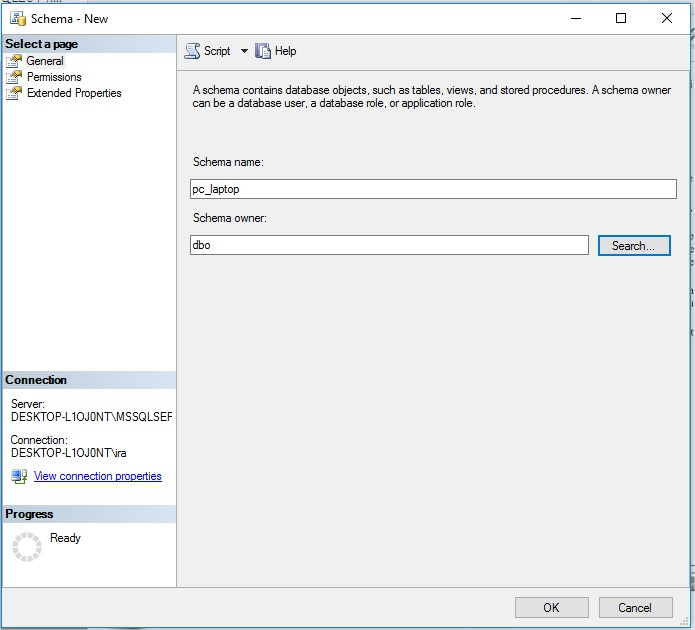
\includegraphics[scale=0.5]{screens/4.jpg}
	\caption*{Figure 3: Defining schema for pc\_laptop}
	\label{}
\end{figure}

\begin{figure}[H]
	\centering
	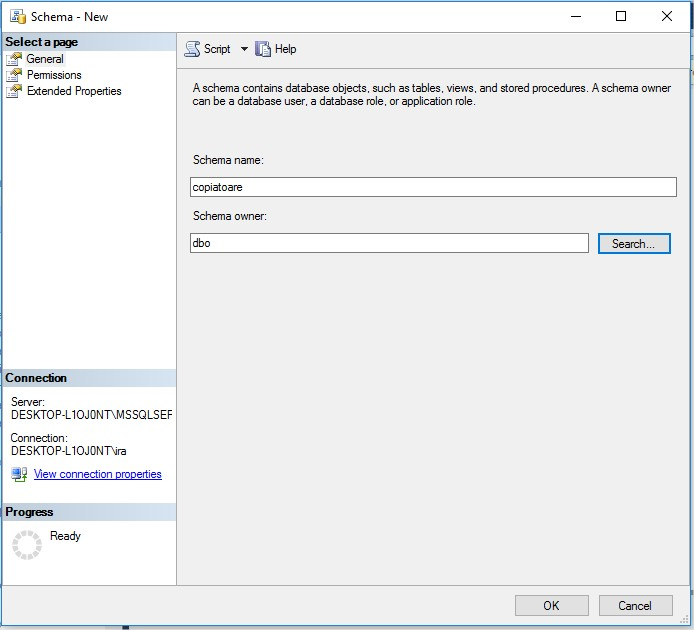
\includegraphics[scale=0.5]{screens/5.jpg}
	\caption*{Figure 4: Defining schema for copiatoare}
	\label{}
\end{figure}

\section{Task 3}
Transferați tabelul produse din schema dbo în schema stoc, ținînd cont de dependențele definite asupra tabelului produse. În același mod să se trateze tabelele pc\_uri, laptop\_uri care aparțin schemei pc\_laptop și imprimante, care aparține schemei copiatoare. Să se scrie instrucțiunile SQL respective.

\begin{figure}[H]
	\centering
		\minipage{0.4\textwidth}
		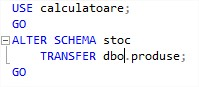
\includegraphics[width=\linewidth]{screens/6.jpg}
		\caption*{Figure 5: Transfering produse to stoc schema}
		\label{}
	\endminipage\hfill
		\minipage{0.4\textwidth}%
		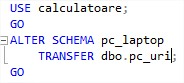
\includegraphics[width=\linewidth]{screens/7.jpg}
		\caption*{Figure 6: Transfering pc\_uri to pc\_laptop schema}
	\endminipage
\end{figure}

\begin{figure}[H]
	\centering
		\minipage{0.4\textwidth}
		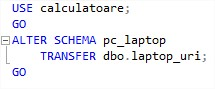
\includegraphics[width=\linewidth]{screens/8.jpg}
		\caption*{Figure 7: Transfering laptop\_uri to pc\_laptop schema}
		\label{}
	\endminipage\hfill
		\minipage{0.4\textwidth}%
		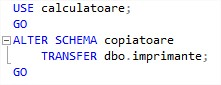
\includegraphics[width=\linewidth]{screens/9.jpg}
		\caption*{Figure 8: Transfering imrimante to copiatoare schema}
	\endminipage
\end{figure}
\bigskip

\section{Task 4}
Modificați interogările asupra bazei de date calculatoare prezentate în capitolul 4 astfel ca numele tabelelor să fie descrise în mod explicit, ținînd cont de faptul că tabelele au fost mutate în scheme noi.

\renewcommand{\labelenumi}{\arabic{enumi})}
\begin{enumerate}
	\item Să se găsească modelul, viteza procesorului și capacitatea discului dur pentru toate pc-urile care costă mai puțin de 500\$. 
	
\begin{figure}[H]
	\centering
		\minipage{0.6\textwidth}
		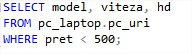
\includegraphics[width=\linewidth]{screens/11.jpg}
		\caption*{Figure 9: Exercise 1}
		\label{}
	\endminipage\hfill
		\minipage{0.35\textwidth}%
		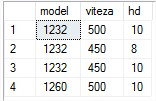
\includegraphics[width=\linewidth]{screens/11ans.jpg}
		\caption*{Figure 10: Answer to exercise 1}
	\endminipage
\end{figure}

	\item Să se găsească producătorii de imprimante.
	
\begin{figure}[H]
	\centering
		\minipage{0.6\textwidth}
		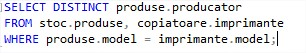
\includegraphics[width=\linewidth]{screens/12.jpg}
		\caption*{Figure 11: Exercise 2}
		\label{}
	\endminipage\hfill
		\minipage{0.28\textwidth}%
		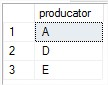
\includegraphics[width=\linewidth]{screens/12ans.jpg}
		\caption*{Figure 12: Answer to exercise 2}
	\endminipage
\end{figure}
\end{enumerate}


\section{Task 5}
Creați sinonimele respective pentru a simplifica interogările costruite în exercițiul precedent și reformulați intergoările, folosind sinonimele create.

\begin{figure}[H]
	\centering
		\minipage{0.48\textwidth}
		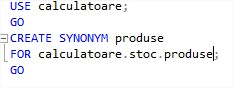
\includegraphics[width=\linewidth]{screens/17.jpg}
		\caption*{Figure 13: Creating synonym for produse}
		\label{}
	\endminipage\hfill
		\minipage{0.48\textwidth}%
		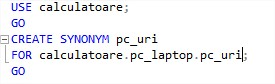
\includegraphics[width=\linewidth]{screens/18.jpg}
		\caption*{Figure 14: Crating synonym for pc\_uri}
	\endminipage
\end{figure}

\begin{figure}[H]
	\centering
		\minipage{0.48\textwidth}
		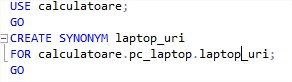
\includegraphics[width=\linewidth]{screens/19.jpg}
		\caption*{Figure 15: Creating synonym for laptop\_uri}
		\label{}
	\endminipage\hfill
		\minipage{0.48\textwidth}%
		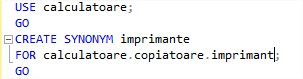
\includegraphics[width=\linewidth]{screens/20.jpg}
		\caption*{Figure 16: Crating synonym for imprimante}
	\endminipage
\end{figure}

In the figures above, I shows how I created the synonyms for the 4 tables. I used the CREATE SYNONYM statement. Also, below we can see the simplified queries that were shown in the previous task.

\renewcommand{\labelenumi}{\arabic{enumi})}
\begin{enumerate}
	\item Să se găsească modelul, viteza procesorului și capacitatea discului dur pentru toate pc-urile care costă mai puțin de 500\$. 
	
\begin{figure}[H]
	\centering
		\minipage{0.7\textwidth}
		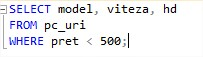
\includegraphics[width=\linewidth]{screens/21.jpg}
		\caption*{Figure 17: Exercise 1}
		\label{}
	\endminipage\hfill
		\minipage{0.28\textwidth}%
		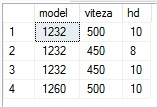
\includegraphics[width=\linewidth]{screens/21ans.jpg}
		\caption*{Figure 18: Answer to exercise 1}
	\endminipage
\end{figure}

	\item Să se găsească producătorii de imprimante.
	
\begin{figure}[H]
	\centering
		\minipage{0.7\textwidth}
		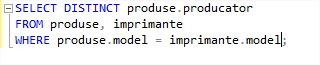
\includegraphics[width=\linewidth]{screens/22.jpg}
		\caption*{Figure 19: Exercise 2}
		\label{}
	\endminipage\hfill
		\minipage{0.28\textwidth}%
		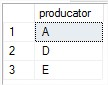
\includegraphics[width=\linewidth]{screens/12ans.jpg}
		\caption*{Figure 20: Answer to exercise 2}
	\endminipage
\end{figure}
\end{enumerate}
\bigskip
